% ============================================================
% Figure 2: Game2Real Domain Adaptation Effect
% Shows feature distribution alignment in t-SNE style
% ============================================================
\documentclass[tikz,border=5pt]{standalone}
\usepackage{tikz}
\usetikzlibrary{shapes,arrows,positioning,fit,backgrounds,calc}
\usepackage{amsmath}

\tikzset{
  point/.style={circle, minimum size=3mm, inner sep=1pt, draw=#1!60, fill=#1!30},
  arrow/.style={->, >=stealth, thick},
}

\begin{document}
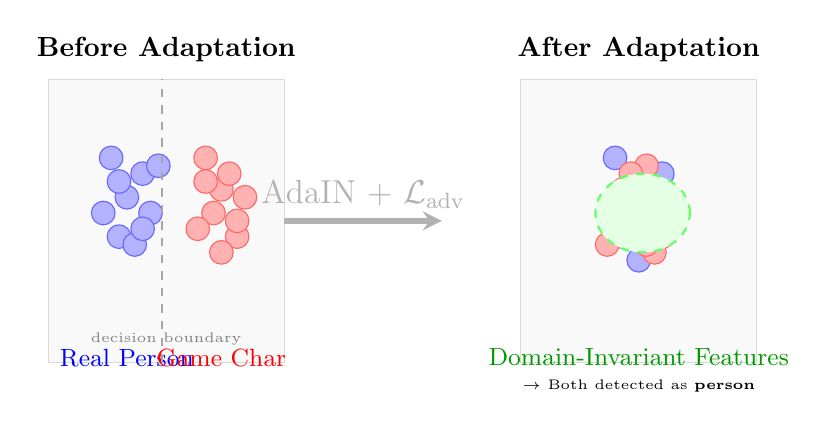
\begin{tikzpicture}[node distance=1.5cm]

% Before adaptation
\begin{scope}[local bounding box=before, shift={(-3.5,0)}]
  \draw[gray!30, fill=gray!5] (-1.5,-1.8) rectangle (1.5,1.8);
  \node[above] at (0,1.9) {\textbf{Before Adaptation}};

  % Real humans (blue cluster)
  \foreach \x/\y in {-0.5/0.3, -0.3/0.6, -0.7/0.8, -0.2/0.1, -0.6/-0.2,
                      -0.8/0.1, -0.1/0.7, -0.4/-0.3, -0.6/0.5, -0.3/-0.1}
    \node[point={blue}] at (\x,\y) {};
  \node[below, font=\small, blue] at (-0.5,-1.5) {Real Person};

  % Game characters (red cluster, far apart)
  \foreach \x/\y in {0.7/0.4, 0.5/0.8, 0.9/-0.2, 0.6/0.1, 0.8/0.6,
                      0.4/-0.1, 1.0/0.3, 0.5/0.5, 0.9/0.0, 0.7/-0.4}
    \node[point={red}] at (\x,\y) {};
  \node[below, font=\small, red] at (0.7,-1.5) {Game Char};

  % Decision boundary
  \draw[dashed, thick, gray!70] (-0.05,-1.8) -- (-0.05,1.8);
  \node[below, font=\tiny, gray] at (0,-1.3) {decision boundary};
\end{scope}

% Arrow
\draw[arrow, line width=2pt, gray!60] (-2,0) -- node[above, font=\large] {AdaIN + $\mathcal{L}_{\text{adv}}$} (0,0);

% After adaptation
\begin{scope}[local bounding box=after, shift={(2.5,0)}]
  \draw[gray!30, fill=gray!5] (-1.5,-1.8) rectangle (1.5,1.8);
  \node[above] at (0,1.9) {\textbf{After Adaptation}};

  % Real humans (blue)
  \foreach \x/\y in {0.0/0.5, 0.2/0.2, -0.3/0.8, 0.1/-0.1, -0.1/0.3,
                      -0.4/0.1, 0.3/0.6, -0.2/-0.2, 0.0/-0.5, 0.4/0.0}
    \node[point={blue}] at (\x,\y) {};

  % Game characters (red, now mixed in same region)
  \foreach \x/\y in {0.1/0.7, -0.2/0.1, 0.3/-0.2, -0.1/0.6, 0.2/-0.4,
                       -0.3/-0.1, 0.4/0.3, -0.2/0.4, 0.1/-0.3, -0.4/-0.3}
    \node[point={red}] at (\x,\y) {};

  % Overlapping region indicator
  \draw[ellipse, draw=green!60, thick, dashed, fill=green!10] (0.05,0.1) ellipse (0.6 and 0.5);
  \node[below, font=\small, green!60!black] at (0.0,-1.5) {Domain-Invariant Features};
  \node[below, font=\tiny] at (0.0,-1.9) {$\rightarrow$ Both detected as \textbf{person}};
\end{scope}

\end{tikzpicture}
\end{document}
